%
% main.tex -- Paper zum Thema Eis
%
% (c) 2018, Silvio Marti, Hochschule Rapperswil
%
\chapter{Eis\label{chapter:eis}}
\lhead{Eis}
\begin{refsection}
\chapterauthor{Silvio Marti}

\section{Einleitung}
\rhead{Einleitung}
Diese Arbeit befasst sich damit, wie die Anwesenheit von Eis an den Polen modelliert werden kann. Immer wieder hört man, dass das Polareis rasant schmilzt und der Eisschwund ein bedrohliches Ausmass angenommen hat. Als Grund wird jeweils die globale Erwärmung genannt. Das scheint plausibel, denn wie man schon im Modell von Budyko \hl{Verweis auf Skript Budyko} sehen kann, gilt für eine höhere Gleichgewichtstemperatur eine tiefere Albedo $a$, was bedeutet, dass es weniger reflektierendes Eis geben muss. Es sei aber betont, dass die Funktion $a(T)$ \hl{Verweis auf Skript Funkion $a(T)$} sich nur auf die beiden Punkte {\em Snowball earth} ($T=250K$, $a=0.7$) und {\em kein Eis} ($T=280K$, $a=0.3$) stützt und dazwischen mit einer willkürlich gewählten $\tanh$ Funktion modelliert wurde. 
\subsection{Eisschmelze am Nordpol}
\rhead{Eisschmelze am Nordpol}
Um eine Idee über das Ausmass der Eisschmelze in den letzten 25 Jahren zu bekommen, dient Abbildung \ref{skript:eis:fig:NASAohne}.
\begin{figure}
	\centering
	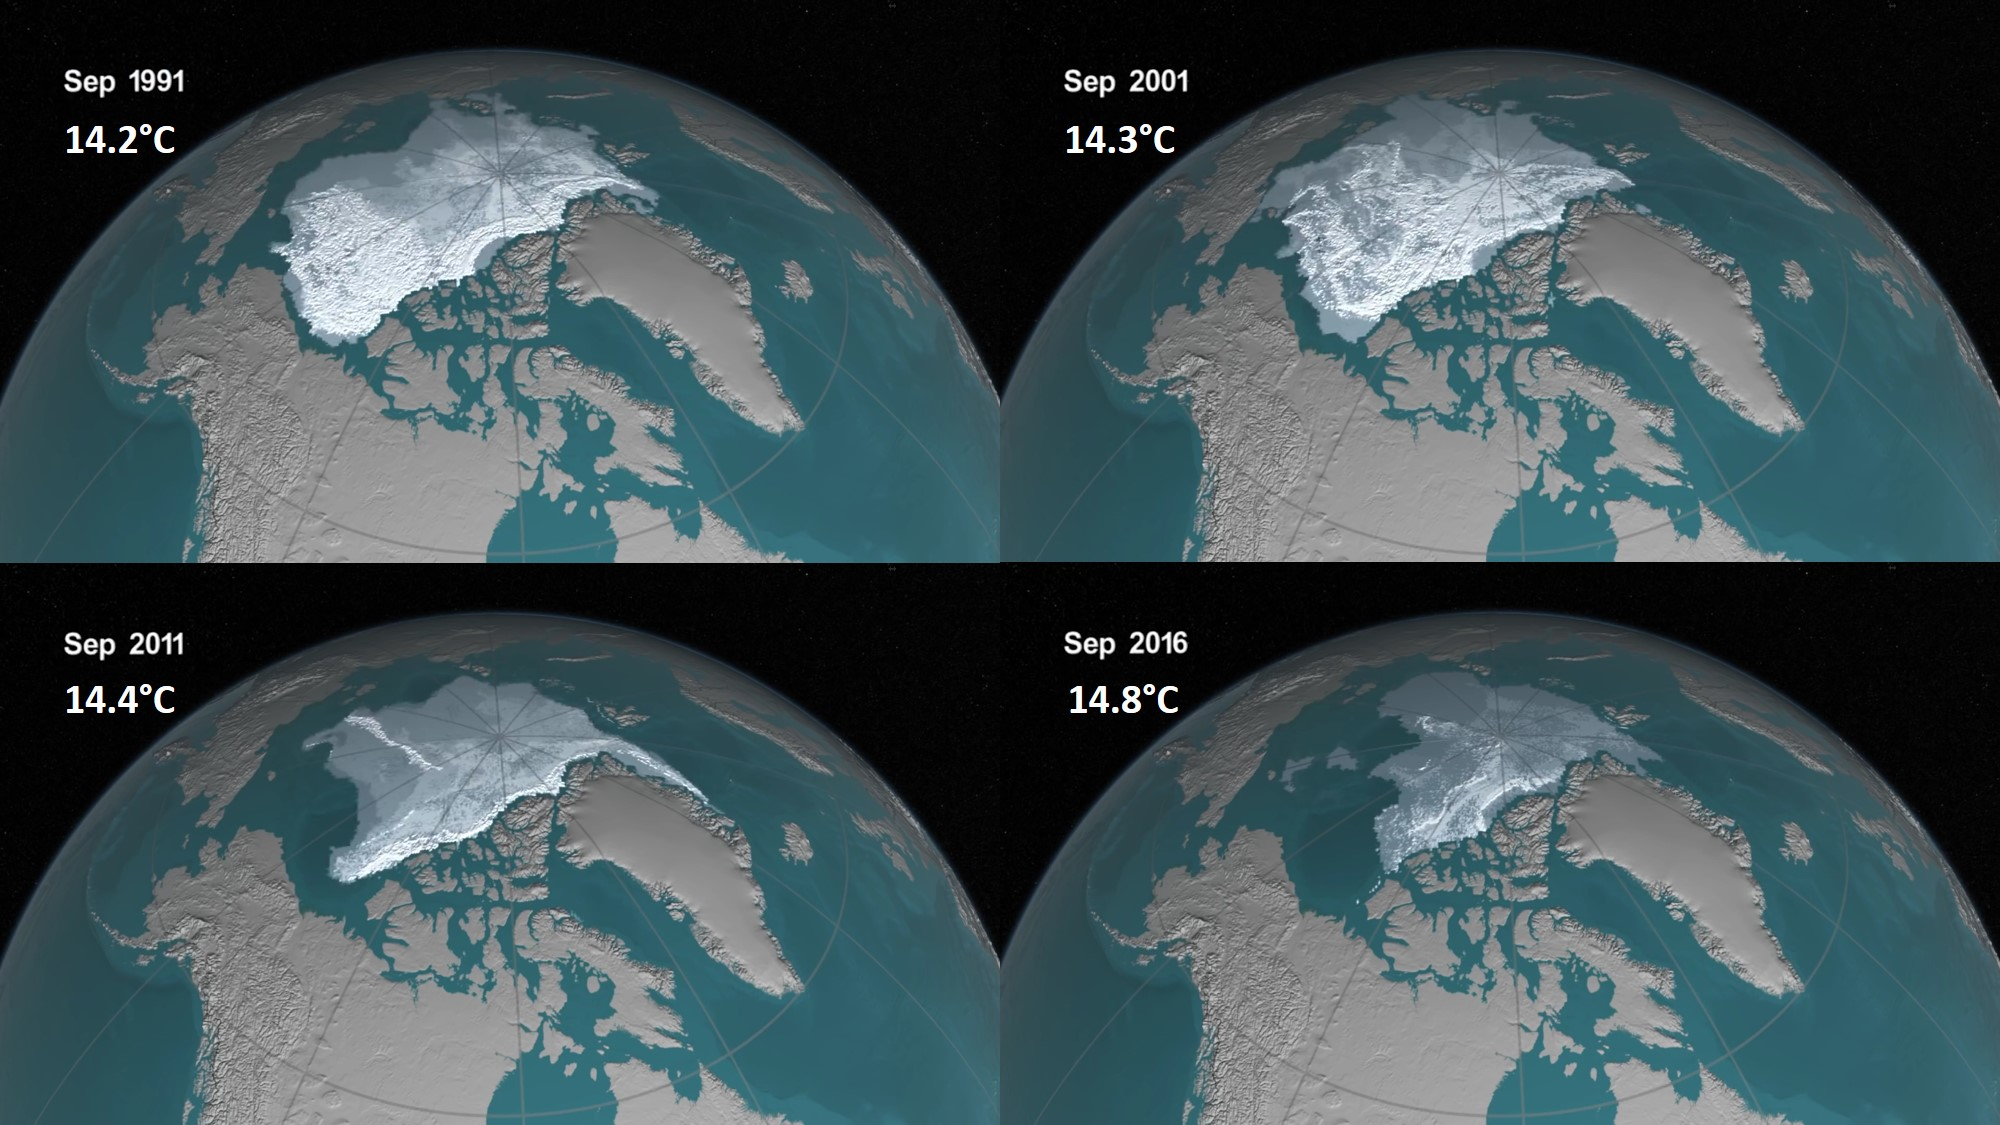
\includegraphics[width=14cm]{eis/NASA_ohne_Breitengraden.jpg}
	\caption{Ausschnitt aus einer Animation der NASA \cite{skript:eis:animation_NASA}. Dargestellt ist das Polareis (nur das Meereis, ganz Grönland ist z.B. auch vereist) jeweils im September des angegebenen Jahres. Je weisser das Eis, desto älter ist es (ganz weiss entspricht vier Jahre und älter).	Dazu ist auch die globale Jahresdurchschnittstemperatur eingetragen.}
	\label{skript:eis:fig:NASAohne}
\end{figure}
Die Abbildung \ref{skript:eis:fig:globale_Mitteltemperaturen} zeigt die Veränderung der globalen Durchschnittstemperatur über einen ähnlichen Zeitraum. Obwohl es wenig Sinn macht, die Temperaturwerte absolut anzugeben, wollen wir das hier tun; wir sehen in Abschnitt \ref{skript:eis:Resultate} die Verwendung. Der Vergleichspunkt, um aus den differenziellen Werten \cite{skript:eis:vitalsign_NASA} absolute zu bekommen, ist das Jahr 2017, in welchem die Temperatur 14.7°C \cite{skript:eis:ref2017} betragen haben soll.
\begin{figure}
	\centering
	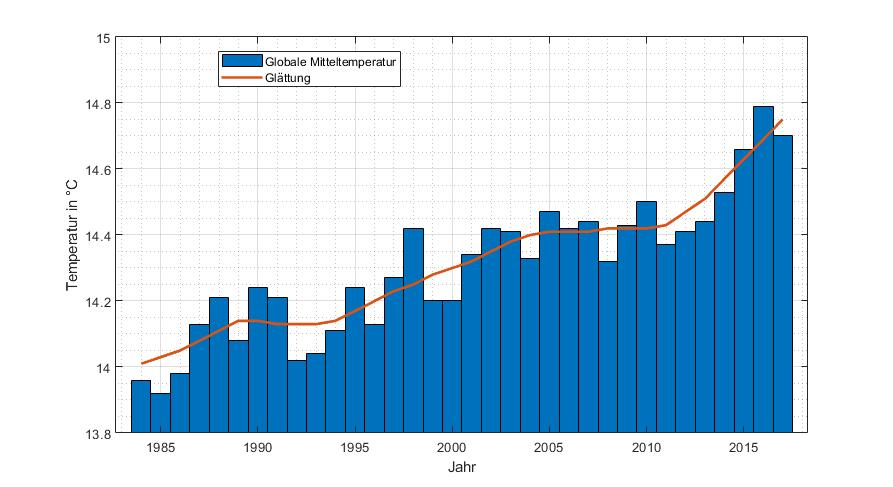
\includegraphics[width=14cm]{eis/globale_Mitteltemperaturen.jpg}
	\caption{Globale Jahresdurchschnittstemperatur 1984 bis 2017}
	\label{skript:eis:fig:globale_Mitteltemperaturen}
\end{figure}
\subsection{Problem an der Eisschmelze} \label{skript:eis:Problem an der Eisschmelze}
\rhead{Problem an der Eisschmelze}
Warum ist den Polkappen eine so grosse Bedeutung für das Klima zuzuschreiben? Folgen für das Klima einer grossen Eisschmelze aufgrund einer Temperaturerhöhung sind unter Anderem: 
\begin{itemize}
	\item Wenn das Eis schmilzt, kommt irgendwann der darunterliegende Boden zum Vorschein. Das führt dazu, dass die Albedo an diesen Stellen sofort um mehr als die Hälfte sinkt, was bedeutet, dass global betrachtet die aufgenommene Strahlungsleistung zunimmt und die Erwärmung weiter vorangetrieben wird.
	\item Taut Permafrost auf, gelangen grosse Mengen des Klimagases Methan, welches zuvor im Permafrost eingeschlossen war, in die Atmosphäre, was ebenfalls zu einer zusätzlichen Erwärmung führt.
\end{itemize}
Veränderungen der Eismenge verstärken sich also von selbst.
Die Eisschmelze ist somit ein Prozess mit einer Mitkopplung mit globalen Auswirkungen.

Entscheidend für die genannten Prozesse ist nicht die Dicke des Eises, sondern nur die Fläche. Wie in Abbildung \ref{skript:eis:fig:NASAohne} zu erkennen ist, befindet sich das Eis ungefähr innerhalb eines Kreises um die Pole.
\begin{definition}
	Der Begriff {\em ice line} oder {\em Eislinie} meint denjenigen Breitengrad, wo die Grenze der Vereisung ist.
	\index{ice line}%
	\index{Eislinie}%
	Alle darüber liegenden Breitengrade sind als vereist zu betrachten, die darunter nicht.
	\label{skript:def:iceline}
\end{definition}
\section{Ziel}
\rhead{Ziel}
Offensichtlich existiert ein Zusammenhang zwischen der globalen Temperatur und der vorhandenen Eisfläche bzw. der Eislinie. Das Ziel ist, einen mathematischen Zusammenhang zu finden, um Aussagen über zukünftige Entwicklungen zu machen.
\section{Von Budyko zur zonalen Energiebilanz}
\rhead{Von Budyko zur zonalen Energiebilanz}
Budykos Modell konnte die Eisschmelze an den Polen nicht darstellen, bzw. aufgrund der nur geschätzten $a(T)$ \hl{Verweis auf Skript Funktion $a(T)$} Funktion keine präzise Aussage über die vorhandene Eisfläche machen. Das Problem besteht darin, dass in diesem Modell einige globale Annahmen getroffen wurden, die nachfolgend identifiziert und manche verbessert werden.
\begin{itemize}
	\item Gleichmässige Einstrahlung. In Budykos Modell trifft das Sonnenlicht auf der gesamten Erdoberfläche mit derselben Intensität auf. Diese Annahme entspricht offensichtlich nicht der Realität, weil das Sonnenlicht nicht überall senkrecht auftrifft. Die ortsabhängige Intensität der Sonneneinstrahlung muss deshalb berücksichtigt werden.
	\item Gleichmässige Eisverteilung. Die grossen Eisflächen konzentrieren sich nur auf die Polargebiete, entsprechend wird nur dort Sonnenlicht reflektiert. Weil die Einstrahlung auch nicht gleichmässig ist, wird wichtig, welche Teile der Erdoberfläche von Eis bedeckt sind. Die Albedo soll deshalb abhängig vom Breitengrad und der Eislinie sein.
	\item Gleichmässige Land- und Wasserverteilung. Budykos Modell geht davon aus, dass die Landmassen auf der Erdoberfläche gleich verteilt sind. Das ist spielt bei der Vereisung eine Rolle, weil sich auf dem Land schneller Eis bildet als auf dem Meer. Besonders der Unterschied von der Nord- und Südhalbkugel ist von Bedeutung.
	\item Gleichmässige Temperaturverteilung. Auf der Erde sind grosse regionale Temperaturunterschiede auszumachen. Weil die abgestrahlte Leistung proportional zu $T^4$ ist, wird nicht überall gleich viel Leistung abgestrahlt. Diese Tatsache werden wir hier aber nicht berücksichtigen.
\end{itemize}
Wir möchten nun Budykos Modell in ein realistischeres überführen, in dem wir die Erde in Zonen (Breitengrade) aufteilen und obige Überlegungen zonenabhängig durchführen.
\subsection{Einstrahlung abhängig vom Breitengrad}
Die eintreffende Energie pro Fläche ist, wie in Abbildung \ref{skript:einfallswinkel} ersichtlich, abhängig vom Einstrahlungswinkel, der dem Breitengrad $\vartheta$ entgegengesetzt ist. Die Energie pro Fläche ist somit proportional zu $\cos(\vartheta)$. Um der Tatsache Rechnung zu tragen, dass die Gegenden um den Äquator mehr Energie als die polaren Regionen erhalten, führen wir die breitengradabhängige Energieverteilungsfunktion
\begin{equation}\label{skript:eis:Energieverteilung Breitengrad}
s(\vartheta)
=
\frac{2}{\pi^2}\int_{0}^{2\pi}\cos(\vartheta)\,d\phi,\quad
\vartheta\in(-\tfrac{1}{2}\pi,\tfrac{1}{2}\pi)
\end{equation}
ein. Der Faktor $\frac{2}{\pi^2}$ wird für die Normalisierungsbedingung in Abschnitt \ref{skript:eis:Modellverbesserung:Normalisierung} verwendet. Wird wie hier nur der Breitengrad berücksichtigt, ergibt sich eine Energieverteilung gemäss Abbildung \ref{skript:eis:fig:Einstrahlung_abh_vom_Breitengrad}.
\begin{figure}
 	\centering
 	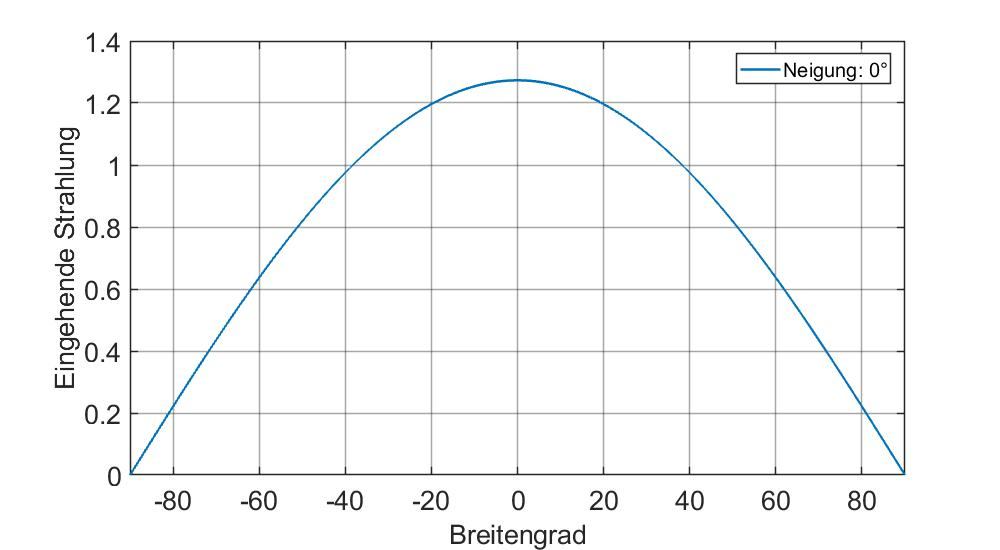
\includegraphics[width=10cm]{eis/Einstrahlung_abh_vom_Breitengrad.jpg}
 	\caption{Energieverteilung abhängig vom Breitengrad $\vartheta$}
 	\label{skript:eis:fig:Einstrahlung_abh_vom_Breitengrad}
\end{figure}
\subsection{Einstrahlung in Abhängigkeit vom Neigungswinkel}
Weil die Erdachse einen Neigungswinkel hat, geht die Sonne im Sommer im hohen Norden nicht unter, was bedeutet, dass auch die Pole Einstrahlung erhalten. Abbildung \ref{skript:eis:fig:Einstrahlung_abh_vom_Breitengrad} kann somit nicht stimmen, die Neigung $\eta$ muss berücksichtigt werden. Um dem Rechnung zu tragen, führen wir den Index $\eta$ ein und schreiben ab jetzt $s_{\eta}(\vartheta)$. Die Energieverteilungsfunktion ist jetzt gegeben durch ein elliptisches Integral
\begin{equation}\label{skript:eis:Energieverteilung Neigung}
s_{\eta}(\vartheta)
=
\frac{2}{\pi^2}\int_{0}^{2\pi}\sqrt{1-(\cos\vartheta\sin\eta \cos\phi-\sin\vartheta \cos\eta)^2}\,d\phi,
\end{equation}
welches in Kapitel \hl{Verweis Skript Kap 5} erläutert wurde. Es kann gezeigt werden, dass die Formel \eqref{skript:eis:Energieverteilung Breitengrad} der Spezialfall von \eqref{skript:eis:Energieverteilung Neigung} für eine Neigung von $0^{\circ}$ ist. Zurzeit beträgt die Neigung $\eta=23.4^{\circ}$, damit verändert sich die Energieverteilung, wie in Abbildung \ref{skript:eis:fig:Einstrahlung_abh_mit_und_ohne_Neigung} zu sehen ist.
\begin{figure}
	\centering
	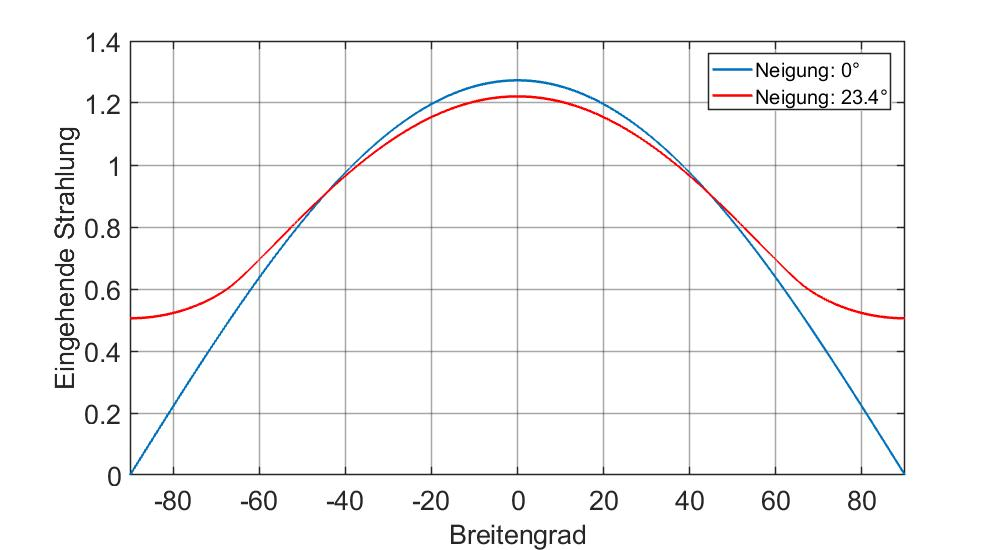
\includegraphics[width=10cm]{eis/Einstrahlung_abh_mit_und_ohne_Neigung.jpg}
	\caption{Energieverteilung abhängig vom Breitengrad $\vartheta$ und dem Neigungswinkel $\eta$}
	\label{skript:eis:fig:Einstrahlung_abh_mit_und_ohne_Neigung}
\end{figure}
Wichtig zu sehen ist hier, dass die Energie an den Polen eben nicht $0$ ist, der Einfluss der Neigung ist somit beträchtlich.

Die saisonalen Schwankungen der Eislinie betragen über ein Dutzend Breitengrade. Aufgrund der Überlegungen über die Neigung wird jetzt auch klar, für welche Jahreszeit wir die Eislinie berechnen wollen. Im Winter, wenn keine Einstrahlung am Nordpol statt findet, wird auch keine Energie vom Eis reflektiert, dessen Ausbreitung verliert also im Winter an Bedeutung. Relevant für unser Modell ist deshalb nur das Eis im Sommer. Weil es zu Beginn jeweils noch viel Eis vom Winter übrig hat, legen wir uns auf den Monat September fest, wo die Ausbreitung ihr Minimum erreicht. Sämtliche Resultate werden sich also auf den Spätsommer beziehen und geben die minimale jahreszeitenabhängige Vereisung an.
\subsection{Normalisierungsbedingung} \label{skript:eis:Modellverbesserung:Normalisierung}
Bei den verwendeten Formeln muss sichergestellt werden, dass die eingestrahlte Leistung immer dieselbe ist. Sie darf nur verteilt, aber nicht verändert werden. Dies lässt sich sicherstellen, indem $s_\eta(\vartheta)$ die Gleichung
\begin{equation}\label{skript:eis:Normalisierungsbedingung}
	\frac{1}{2}\int_{-\pi/2}^{\pi/2}s_{\eta}(\vartheta)\cos\vartheta\,d\vartheta
	=
	1
\end{equation}
erfüllen muss. Weil die Fläche einer normierten positiven Cosinushalbwelle $2$ ist, wird dies hier mit dem Faktor $\tfrac{1}{2}$ auf $1$ korrigiert.
\subsection{Approximation der Energieverteilung}
Für die breitengradabhängige Einstrahlung erweist es sich als mühsam, die Formel \eqref{skript:eis:Energieverteilung Neigung} zu benutzen, weil für jeden Breitengrad das Integral aufgelöst werden muss. Die Funktion soll deshalb für eine fixe Neigung von $\eta=23.4^{\circ}$ approximiert werden. Dazu wird eine Fourier-Analyse gemäss Kapitel \ref{chapter:fourier} durchgeführt. Weil die Funktion symmetrisch ist, entfallen alle Sinus- sowie die ungeraden Cosinusterme. Es scheint gemäss Abbildung \ref{skript:eis:fig:Einstrahlung_abh_mit_und_ohne_Neigung} besonders die Frequenz $2\tfrac{\text{rad}}{\text{s}}$ stark vertreten zu sein, höhere Frequenzen sind aufgrund des flachen Kurvenverlaufs kaum zu erwarten. Wir versuchen deshalb, \eqref{skript:eis:Energieverteilung Neigung} mit
\begin{equation}\label{skript:eis:Energieverteilung Approximation}
	\tilde{s}(\vartheta)
	=
	s_0+s_1\cos(2\vartheta)
\end{equation}
zu approximieren.
Selbstverständlich muss auch die Approximation die Normalisierungsbedingung \eqref{skript:eis:Normalisierungsbedingung} erfüllen, was der Fall ist, wenn wir $s_0=0.881$ und $s_1=0.358$ wählen.
Wie in Abbildung \ref{skript:eis:fig:Einstrahlung_approximiert_Vergleich} zu sehen ist, deckt sich die Approximation bereits so gut mit der Originalfunktion, dass auf höherfrequente Cosinusterme verzichtet wird.
\begin{figure}
	\centering
	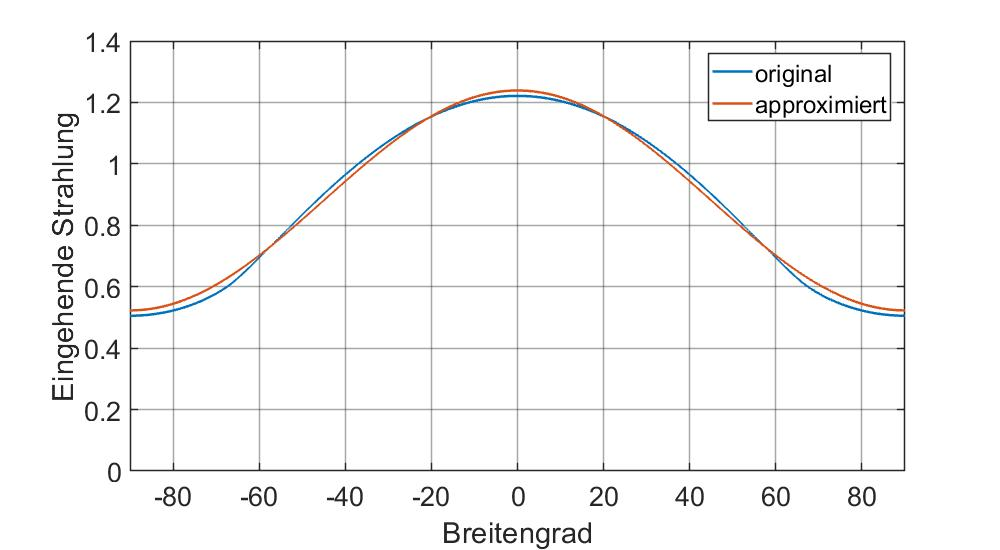
\includegraphics[width=10cm]{eis/Einstrahlung_approximiert_Vergleich.jpg}
	\caption{Vergleich der Energieverteilungsfunktion gemäss \eqref{skript:eis:Energieverteilung Neigung} mit der Approximation \eqref{skript:eis:Energieverteilung Approximation}}
	\label{skript:eis:fig:Einstrahlung_approximiert_Vergleich}
\end{figure}
\subsection{Absorbtionsverteilung}
In den vereisten Breitengraden wird mehr Sonnenlicht reflektiert, die Albedo ist deshalb dort grösser als bei einer nicht vereisten Oberfläche. Gemäss der Definition in Abschnitt \ref{skript:def:iceline} ergibt sich für die Albedo
\begin{equation}\label{skript:eis:Albedoverteilung}
a(\vartheta,\vartheta_\text{iceline})
=
\left\{
\begin{tabular}{lll}
	$a_\text{Eis}$&$-\tfrac{\pi}{2}\leq\vartheta\leq-\vartheta_\text{iceline}$&$\text{Südpolarkappe}$\\
	$a_\text{Land}$&$-\vartheta_\text{iceline}\leq\vartheta\leq\vartheta_\text{iceline}$&$\text{Äquatorialzone}$\\
	$a_\text{Eis}$&$\vartheta_\text{iceline}\leq\vartheta\leq\tfrac{\pi}{2}$&$\text{Nordpolarkappe}$
\end{tabular}
\right.,
\end{equation}
wobei wir die Parameter $a_\text{Eis}=0.7$ und $a_\text{Land}=0.285$ wählen. Diese Funktion ist in Abbildung \ref{skript:eis:fig:Albedoverteilung} dargestellt.
\begin{figure}
	\centering
	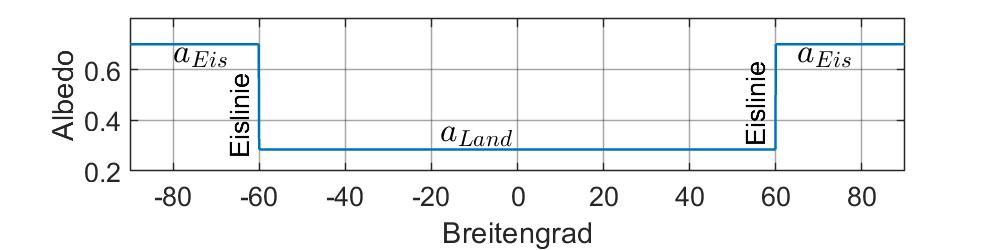
\includegraphics[width=10cm]{eis/Albedo_abh_Breitengrad.jpg}
	\caption{Veranschaulichung der Gleichung \eqref{skript:eis:Albedoverteilung} für eine Eislinie bei $60^\circ$.}
	\label{skript:eis:fig:Albedoverteilung}
\end{figure}
\section{Energiegleichung}
\rhead{Energiegleichung}
Nun haben wir alle Komponenten zusammen, um sie wieder in Budykos Modell einzufügen. Mit Berücksichtigung der Zonen ergibt sich die Gleichung
\begin{equation}\label{skript:eis:Ein pro Breitengrad}
E_\text{in}(\vartheta,\vartheta_\text{iceline})
=
(1-a(\vartheta,\vartheta_\text{iceline}))\cdot\tilde{s}_{b}(\vartheta)\cdot Q
\end{equation}
für die eingehende Strahlung pro Breitengrad, wobei $Q=\tfrac{1}{4}S_{0}$. Damit die gesamte einfallende Energie betrachtet werden kann, muss die Gleichung \eqref{skript:eis:Ein pro Breitengrad} über alle Breitengrade integriert werden. Dafür wird die Normalisierungsbedingung \eqref{skript:eis:Normalisierungsbedingung} verwendet. Wird alles eingesetzt, resultiert
\begin{equation}\label{skript:eis:Ein abh ice line}
E_\text{in}(\vartheta_\text{iceline})
=
\frac{Q}{2}\int_{-\pi/2}^{\pi/2}(1-a(\vartheta,\vartheta_\text{iceline}))\cdot\tilde{s}(\vartheta)\cdot\cos\vartheta\,d\vartheta,
\end{equation}
wobei $E_\text{in}$ nur noch abhängig von der Eislinie ist, was das Ziel war.
Um die Gleichgewichtslösungen zu erhalten, setzen wir $E_\text{in}$ mit $E_\text{out}$ gleich wie in \hl{Verweis Skript Budyko} und bekommen
\begin{equation}\label{skript:eis:Gleichgewichtsgleichung}
	E_\text{in}(\vartheta_\text{iceline})
	=
	\varepsilon\sigma T^4,
\end{equation}
wobei $T$ in $K$ angegeben ist.
\section{Resultate} \label{skript:eis:Resultate}
\rhead{Resultate}
\subsection{Albedo abhängig von der Eislinie}
\rhead{Albedo abhängig von der Eislinie}
\begin{figure}
	\centering
	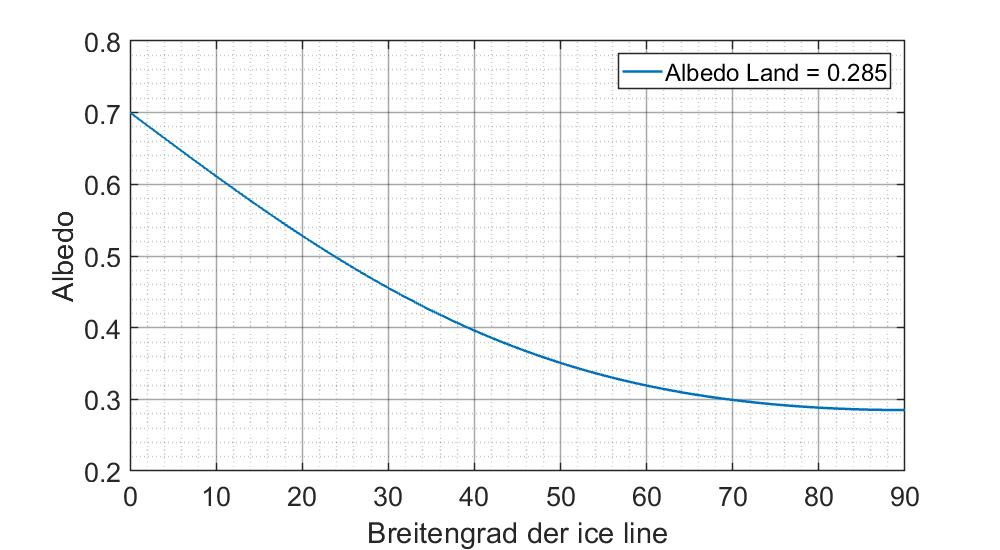
\includegraphics[width=14cm]{eis/Albedo_abh_von_der_ice_line.jpg}
	\caption{Globale Albedo abhängig von der Eislinie. Ist die Erde zugefroren nimmt die globale Albedo den Wert des Eises an, existiert kein Eis, resultiert der Wert des Landes. Reduziert sich die Eismenge, fällt die Albedo monoton.}
	\label{skript:eis:fig:Albedo_abh_von_der_ice_line}
\end{figure}
Die Gleichung der Normalisierungsbedingung \eqref{skript:eis:Normalisierungsbedingung} kann auch dazu verwendet werden, die globale Albedo abhängig von der Eislinie
\begin{equation}
	a(\vartheta_\text{iceline})
	=
	\frac{1}{2}\int_{-\pi/2}^{\pi/2}a(\vartheta,\vartheta_\text{iceline})\cdot\tilde{s}_{\eta}(\vartheta)\cdot\cos\vartheta\,d\vartheta
\end{equation}
zu berechnen. 
Wie schon im Modell von Budyko angenommen, ist in Abbildung \ref{skript:eis:fig:Albedo_abh_von_der_ice_line} klar ersichtlich, dass die Anwesenheit von Eis in den Polregionen nur wenig Einfluss auf die globale Albedo hat. 
\subsection{Eislinie abhängig von der Temperatur}
\rhead{Eislinie abhängig von der Temperatur}
\begin{figure}
	\centering
	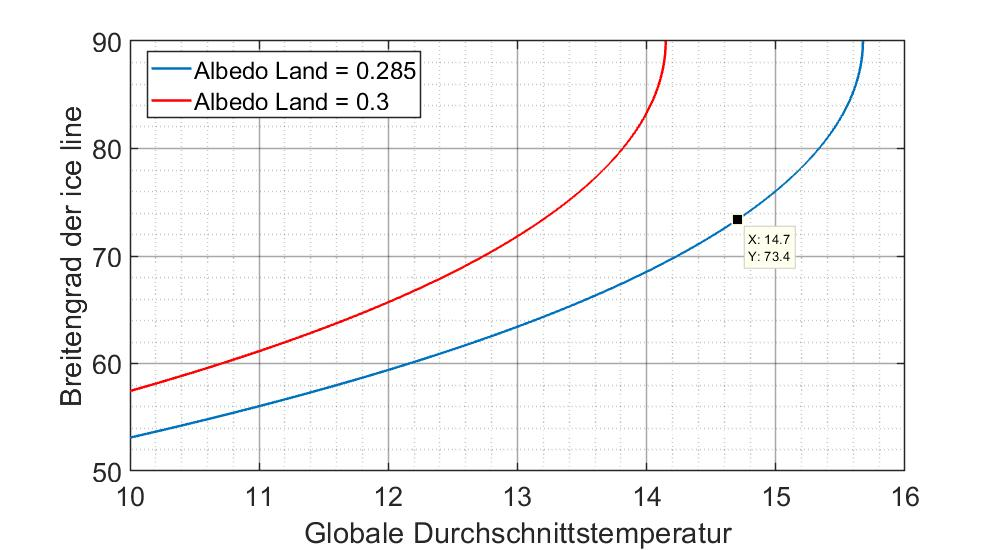
\includegraphics[width=14cm]{eis/iceline_abh_von_der_Temperatur_mit_Verleich_albedo_0,3.jpg}
	\caption{Abhängigkeit der Eislinie von der Temperatur für zwei verschiedene Werte der Land Albedo. Der Messpunkt ist bei der Jahrestemperatur von 2017 eingetragen.}
	\label{skript:eis:fig:iceline_abh_von_der_Temperatur}
\end{figure}
Wird die Gleichgewichtsgleichung \eqref{skript:eis:Gleichgewichtsgleichung} nach der Temperatur $T$ aufgelöst, kann die Eislinie in Abhängigkeit der Temperatur dargestellt werden. Abbildung \ref{skript:eis:fig:iceline_abh_von_der_Temperatur} zeigt, wie sich die Eislinie bei einer globalen Erwärmung verhält. Je weniger Eis vorhanden ist, desto empfindlicher reagiert die Eislinie auf eine Temperaturänderung, bis das Eis fast schlagartig verschwindet.

Hier erklärt sich auch, warum für $a_\text{Land}$ der Wert 0.285 und nicht wie bei Budyko 0.3 verwendet wurde: Das Modell würde uns seit 20 Jahren kein Eis mehr zugestehen, entsprechend musste der Wert so angepasst werden, dass es realistischer wird. Erwärmt sich die Erde weiter wie bis anhin, könnte das Polareis noch in diesem Jahrhundert im Sommer vollständig verschwinden.
\subsection{Eisfläche abhängig von der Temperatur}
\rhead{Eisfläche abhängig von der Temperatur}
Ist die Eislinie bekannt, kann daraus mit
\begin{equation} \label{skript:eis:Eisfläche}
	A_\text{Eis}=2\cdot 2\pi R^2(1-\sin\vartheta)
\end{equation}
die Eisfläche am Nord- und Südpol berechnet werden, wobei $R$ dem Polradius von 6356km entspricht.
\begin{figure}
	\centering
	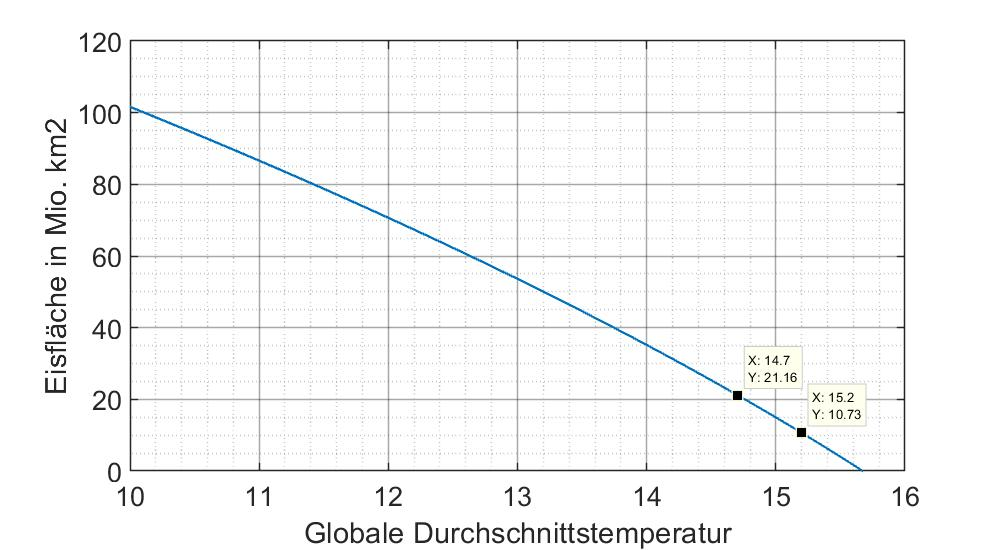
\includegraphics[width=14cm]{eis/Eisflaeche_abh_von_der_Temperatur.jpg}
	\caption{Zusammenhang der globalen Eisfläche und der Durchschnittstemperatur. Die Datenpunkte sind für die Temperatur vom Jahr 2017 und für eine zusätzliche Erwärmung von $0.5^{\circ}$.}
	\label{skript:eis:fig:Eisflaeche_abh_von_der_Temperatur}
\end{figure}
Etwas unerwartet zeigt sich in Abbildung \ref{skript:eis:fig:Eisflaeche_abh_von_der_Temperatur}, dass dieser Zusammenhang beinahe linear ist. Bei einer Erwärmung ausgehend vom Jahr 2017 um weitere $0.5^{\circ}$C werden 10 Mio. km$^2$ Eis schmelzen, was rund $\tfrac{1}{50}$ der Erdoberfläche entspricht. Diese Zahlen stimmen aber so nicht wirklich, weil innerhalb der Eislinie doch nicht alles vereist ist. Sie zeigen aber die drastischen Auswirkungen einer geringen Temperaturerhöhung.
\subsection{Vergleich mit der Realität}
\rhead{Vergleich mit der Realität}
Wie gut stimmt das Modell mit der Realität überein? Wir wollen dafür wieder die Bilder der NASA anschauen und die Daten des Modells einfügen. Dies wurde in Abbildung \ref{skript:eis:fig:NASA_mit_Breitengraden} gemacht.
\begin{figure}
	\centering
	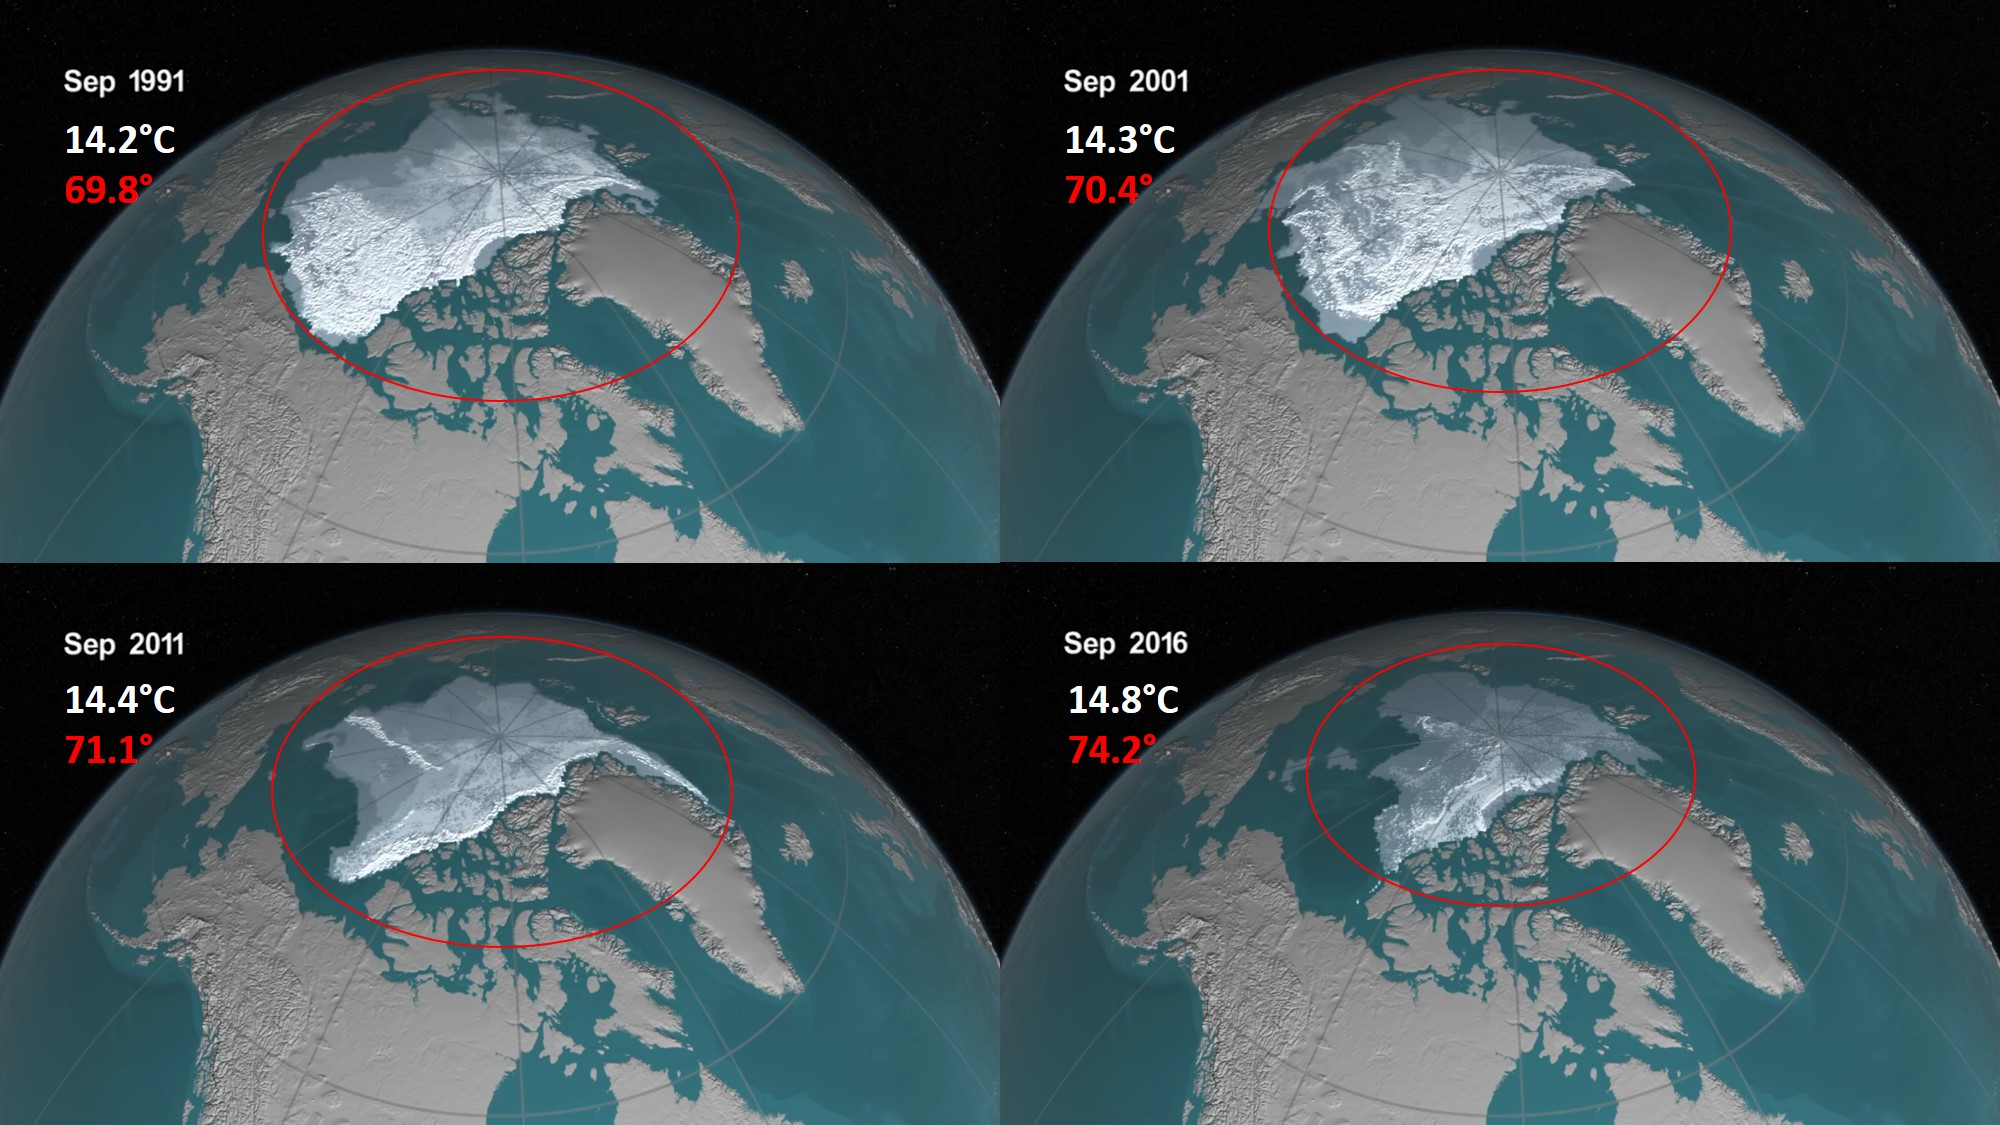
\includegraphics[width=14cm]{eis/NASA_mit_Breitengraden.jpg}
	\caption{Siehe Abb. \ref{skript:eis:fig:NASAohne}.
	Vergleich der Eisflächen mit der für die angegebene Durchschnittstemperatur berechneten Eislinie.}	\label{skript:eis:fig:NASA_mit_Breitengraden}
\end{figure}
Besonders in der Region Alaska und Kanada ist die Übereinstimmung gut, an anderen Orten, wie über Skandinavien, deutlich schlechter, dort hat der Golfstrom einen grossen Einfluss. Zu beachten ist, dass ganz Grönland auch vereist ist. Das Modell kann also die Eisschmelze der letzten Jahre beschreiben, es scheint somit auch für zukünftige Temperaturen brauchbare Prognosen zu liefern.
\section{Modellfehler}
\rhead{Modellfehler}
Obwohl das Modell plausible Resultate liefert, wollen wir hier die Fehler und getroffenen Annahmen diskutieren. Folgende Punkte sind dabei besonders wichtig:
\begin{itemize}
	\item Kein Wärmefluss. Der gesamte Energieaustausch zwischen den Breitengraden in Form von Wärmeleitung und besonders von Konvektion durch die Meeresströmungen (siehe Abbildung \ref{skript:thc:foerderband}), wurde unterbunden. So führt beispielsweise der Golfstrom dazu, dass es in Skandinavien weniger Permafrost und oberhalb weniger Meereis gibt, als in vergleichbaren Regionen.
	\item Symmetrie (ungleiche Land- und somit Eisverteilung zwischen der Nord- und Südhalbkugel). Landflächen vereisen einfacher bis in tiefe Breitengrade als Meer, weil die fehlende Strömung zu weniger Wärmetransport an die Oberfläche führt. In der Folge bildet sich auf dem Land bereits ab etwa dem 55. Breitengrad Permafrost. Auf der Nordhalbkugel hat es in den Breitengraden von $55^\circ$ bis $70^\circ$ bedeutend mehr Landfläche als auf der Südhalbkugel, deshalb darf dort mit mehr Eis gerechnet werden. So sind grosse Gebiete wie Teile von Kanada, Alaska, Sibirien und Skandinavien auch im Sommer gefroren, wo es im Vergleich zur Antarktis kein Eis gibt.
	\item Die abgestrahlte Leistung ist auch temperatur- und somit breitengradabhängig. Indem wir Zonen mit und ohne Eis und eine globale Durchschnittstemperatur über $0^\circ\text{C}$ haben, lassen wir implizit unterschiedliche Oberflächentemperaturen zu. Weil die abgestrahlte Leistung proportional zu $T^4$ ist, wird an den Polen bestimmt nicht gleich viel Energie abgestrahlt, wie am Äquator.
	\item Kein Wärmespeichereffekt. Dies führt dazu, dass keine Jahreszeiten abgebildet werden können; die Eislinie schwankt über das Jahr um über ein Dutzend Breitengrade. Das Eis mittelt Temperaturschwankungen auch über mehrere Jahre aus.
	\item Approximationen. Zu guter Letzt sei erwähnt, dass die Energieverteilung mit der Gleichung \eqref{skript:eis:Energieverteilung Approximation} approximiert wurde. Der Einfluss auf das Ergebnis dürfte aufgrund der guten Übereinstimmung mit \eqref{skript:eis:Energieverteilung Neigung} aber gering ausfallen.
\end{itemize}
\section{Schlussfolgerung}
\rhead{Schlussfolgerung}
\begin{itemize}
	\item Es kann ein einfaches Modell berechnet werden, welches einen Zusammenhang zwischen der Eislinie und der globale Durchschnittstemperatur herstellt.
	\item Das Modell kann die Veränderungen der Eislinie der letzten Jahre aufgrund der Temperaturerhöhung plausible wiedergeben.
	\item Die Eislinie reagiert sehr empfindlich auf eine Temperaturänderung. Bei der Eisfläche sieht es weniger schlimm aus. 
\end{itemize}
Mit Sicherheit kann gesagt werden, dass das Eis an den Polen zukünftig noch mehr zurückgehen wird, wenn sich die Erde weiterhin erwärmt. Es ist denkbar, dass wir einmal einen im Sommer eisfreien Nordpol noch erleben könnten. Die gute Nachricht dabei: Das Modell macht keine Aussage darüber, dass der Prozess der Eisbildung nicht reversibel wäre. Sollte sich die Erde also wieder abkühlen, wird es wieder mehr Eis geben, andernfalls ist aber mit einem massiven Anstieg des Meeresspiegels und der damit verbundenen Flutung von Küstenstädten und ganzen Inseln zu rechen.
\printbibliography[heading=subbibliography]
\end{refsection}
